%*****************************************
\chapter{Validating \tlaplus SMT proof}\label{ch:tla}
%*****************************************


\begin{figure}[t]
    \centering
    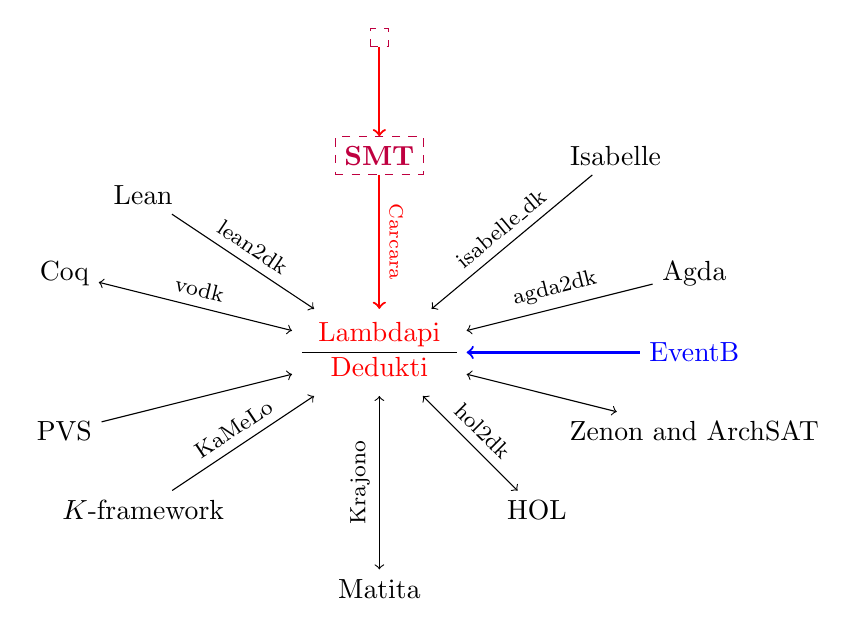
\begin{tikzpicture}
      \path (0,0) node (lp) {\begin{tabular}{c}
        \textcolor{red}{Lambdapi} \\
        \hline
        \textcolor{red}{Dedukti}
      \end{tabular}}
            (-4,1) node (coq) {Coq}
            (-3,2) node (lean) {Lean}
            (0,2.5) node [draw, dashed, purple] (smt) {\color{purple}\textbf{SMT}}
            (0,4) node [draw, dashed, purple] (tla) {\color{purple}\tlaplus}
            (3,2.5) node (isa) {Isabelle}
            (4,1) node (agda) {Agda}
            (-3,-2) node (k) {$\mathbb{K}$-framework}
            (0,-3) node (mat) {Matita}
            (2,-2) node (hol) {HOL}
            (-4,-1) node (pvs) {PVS}
            (4,0) node (eventb) {\textcolor{blue}{EventB}}
            (4,-1) node (ze) {Zenon and ArchSAT}
            ;
      \draw[->,red, thick] (smt) -- (lp) node[midway,sloped,above]
      {\scriptsize{Carcara}};
      \draw[->,red, thick] (tla) -- (smt) node[midway,sloped,above] {};
      \draw[->,blue, thick] (eventb) -- (lp) node[midway,sloped,above] {};
      \draw[->] (lean) -- (lp) node[midway,sloped,above] {\footnotesize{lean2dk}};
      \draw[->] (isa) -- (lp) node[midway,sloped,above] {\footnotesize{isabelle\_dk}};
      \draw[->] (agda) -- (lp) node[midway,sloped,above] {\footnotesize{agda2dk}};
      \draw[<->] (ze) -- (lp) node[midway,sloped,above] {};
      \draw[<->] (hol) -- (lp) node[midway,sloped,above] {\footnotesize{hol2dk}};
      \draw[<->] (mat) -- (lp) node[midway,sloped,above] {\footnotesize{Krajono}};
      \draw[->] (pvs) -- (lp);
      \draw[->] (k) -- (lp) node[midway,sloped,above] {\footnotesize{KaMeLo}};
      \draw[<->] (coq) -- (lp)  node[midway,sloped,above] {\footnotesize{vodk}};
    \end{tikzpicture}
    \caption{Verifying TLAPS proof with Lambdapi.}
    \label{fig:interop-tla}
\end{figure}

\tlaplus is a specification language based on the Temporal Logic of Actions and Zermelo–Fraenkel set theory with the Axiom of Choice (ZFC) \cite{tlabook,tla-ref}.
It is particularly used for specifying concurrent and distributed systems.
The \tlaplus Proof System (TLAPS) extends the language with a formal proof syntax and a tactical proof language \cite{tla-proofs}.

TLAPS includes a \emph{Proof Manager} that decomposes proofs into individual proof obligations, which are then dispatched to various backend provers.
These currently include Isabelle/\tlaplus \cite{isabelle-hol-ref}, Zenon \cite{zenonmodulo},
the SMT solvers cvc5 \cite{cvc5}, veriT \cite{verit} and Z3 \cite{z3}, and finally the LS4 prover for temporal logic.
Each obligation is translated into the logic supported by the corresponding backend.
For SMT solvers \cite{new-encoding-tlaps}, the supported logics include \textbf{UF}, \textbf{LIA}, and \textbf{NIA}.
At present, TLAPS does not verify the correctness of solver outputs, except in the case of Zenon, whose proofs can be independently validated by Isabelle,
and in the case of Isabelle/\tlaplus backend.

As the \cref{fig:interop-tla} suggests, the previous work discussed in \cref{ch:reconstruction} can be leveraged to verify \tlaplus proofs from the SMT solver backend.
The proposed approach involves extracting the output generated by the SMT backend, retrieving the corresponding proof from cvc5 or veriT, and reconstructing it within Lambdapi to establish its validity.

% \section{Overview of TLAPS’s Encoding for SMT Solvers}
% \label{sec:tlaps-encoding-smt}

% \begin{align}
%     &\mathop{\mathtt{ASSUME}}~\mathop{\mathtt{NEW}}~n \in Nat \\
%     &\quad \mathop{\mathtt{PROVE}} \quad (0 \dots n) \cup \{ n + 1 \} = 1 \dots (n+1)
% \end{align}

% The keyword $\mathop{\mathtt{ASSUME}}$ precedes a list of declarations (introduced by new) and hypotheses. Here the hypothesis
% $n \in Nat$ is directly introduced with the declaration of $n$. The keyword  $\mathop{\mathtt{PROVE}}$ precedes the goal.
% Many primitive constructs of \tlaplus are standard mathematical notations. $i \dots j$ denotes the set of integers between $i$ and $j$.
% Given this obligation, the original SMT encoding will produce an equivalent formula in multi-sorted first-order logic, like this one:

% \begin{equation*}
% \forall n^{\kw{int}}, n \geq 0 \Rightarrow \forall i^{\kw{int}}, (1 \leq i \leq n) \lor i = (n+1) \Leftrightarrow 1 \leq i \leq (n + 1)
% \end{equation*}

% Several techniques are used to achieve this result. A powerful type synthesis mechanism attempts to assign sorts to bound variables—here the builtin sort int
% of SMT is assigned to $n$. The obligation is then preprocessed in an attempt to eliminate the \tlaplus primitives with no counterpart in SMT. Since $n$ is an
% $\Z$, both members of the equality are identified as sets of integers, which is why set extensionality is applied.

% \smallskip

% \begin{equation}\label{eq:setext}
%     \forall x, \forall y, (\forall z, z \in x  \Leftrightarrow z \in y) \Leftrightarrow x = y
% \end{equation}

% \begin{lstlisting}[language=SMT, caption={Axiom of extensionality encoded in SMT by TLAPS}, label={setext-lst}]
% (declare-sort Idv 0)
% (declare-fun SetExtTrigger (Idv Idv) Bool)
% (assert
%   (!
%     (forall ((x Idv) (y Idv))
%       (!
%         (=>
%           (forall ((z Idv))
%             (= (Mem z x)
%               (Mem z y))) (= x y))
%         :pattern ((SetExtTrigger x y))))
%     :named |SetExt|))
% \end{lstlisting}

% \smallskip

\section{Validating TLAPS proof}
\label{sec:validating-tlaps-proof}

% -------------- MODULE Cantor1 -----------------
% THEOREM cantor ==
%   \A S :
%     \A f \in [S -> SUBSET S] :
%       \E A \in SUBSET S :
%         \A x \in S :
%           f [x] # A
% PROOF
%   <1>1. TAKE S
%   <1>2. TAKE f \in [S -> SUBSET S]
%   <1>3. DEFINE T == { z \in S : z \notin f[z] }
%   <1>4. WITNESS T \in SUBSET S
%   <1>5. TAKE x \in S
%   <1>6. QED BY x \in T \/ x \notin T
\begin{figure}[tb]
\centering
\begin{nomodule}
\topbar{Cantor}
\[\begin{noj}
  \THEOREM\ cantor\ \deq \\
  \A S : \\
  \quad \A f \in [S \implies \SUBSET\ S] : \\
  \quad\quad \exists A \in \SUBSET\ S : \\
  \quad\quad\quad \forall x \in S : \\
  \quad\quad\quad\quad f \sq{x}{} \mathbin{\#} A \\
  \ps{1}{1.}\ \TAKE\ S \\
  \ps{1}{2.}\ \TAKE\ f \in [S \implies \SUBSET\ S]\\
  \ps{1}{3.}\ \DEFINE\ T\ \deq\ \{ z \in S : z \notin f[z] \}\\
  \ps{1}{4.}\ \WITNESS\ T\ \in \SUBSET\ S \\
  \ps{1}{5.}\ \TAKE\ x \in S \\
  \ps{1}{6.}\ \QED\ \BY\ x \in T \lor x \notin T
\end{noj}\]
\bottombar
\end{nomodule}
\caption{Cantor theorem in \tlaplus}
\label{fig:cantor-tlaps}
\end{figure}

\tlaplus proofs are hierarchically structured and are generally written topdown.
The assertion that the cantor theorem stating that no function ($f$) from a set ($S$) to its power set (\SUBSET\ $S$) can be surjective is formalized in \tlaplus as the theorem in \cref{fig:cantor-tlaps}.
Each proof in the hierarchy ends with a \QED\ step that asserts the proof's goal.
Proofs are incrementally decomposed into simpler subproofs across multiple levels. Each proof consists of labeled steps $\ps{i}{k.}$, that reflect their depth in the proof tree, where level $n$ indicates the nesting depth.
Steps may introduce assumptions, intermediate claims, or invoke previously proven results, using TLAPS tactics such as \ASSUME/\PROVE\, \TAKE\ or \WITNESS.
The proof is completed when the root goal is reduced to a collection of leaf obligations marked as \QED\ and discharged by backend provers.
Besides, TLAPS does not yet handle temporal reasoning.

For each step $\ps{i}{k.}$ in \tlaplus proof, there is a proof obligation that is to be proved.
The obligation contains a context of known facts, definitions, declarations, and a goal.
Obligations are sent to a suitable backend select by the PM (Zenon, Isabelle/TLA, SMT solvers) that tries to prove it.
In the case of \cref{fig:cantor-tlaps}, we will have 6 proof obligations $(\ps{1}{1.} - \ps{1}{6.})$ that will be discharged to the backend.
For example, the proof obligation relative to the final step $\ps{1}{6.}$ is given as follows:

% ===============================================


% ;;	ASSUME NEW CONSTANT CONSTANT_S_,
% ;;	       NEW CONSTANT CONSTANT_f_ \in [CONSTANT_S_ -> SUBSET CONSTANT_S_],
% ;;	       NEW CONSTANT CONSTANT_x_ \in CONSTANT_S_,
% ;;	       CONSTANT_x_
% ;;	       \in {CONSTANT_z_ \in CONSTANT_S_ :
% ;;	              CONSTANT_z_ \notin CONSTANT_f_[CONSTANT_z_]}
% ;;	       \/ CONSTANT_x_
% ;;	          \notin {CONSTANT_z_ \in CONSTANT_S_ :
% ;;	                    CONSTANT_z_ \notin CONSTANT_f_[CONSTANT_z_]} 
% ;;	PROVE  CONSTANT_f_[CONSTANT_x_]
% ;;	       # {CONSTANT_z_ \in CONSTANT_S_ :
% ;;	            CONSTANT_z_ \notin CONSTANT_f_[CONSTANT_z_]}
\begin{figure}[tb]
\centering
\[\begin{noj}
  \quad\begin{noj2}
    \ASSUME & \NEW\ \CONSTANT\ S, \\
            & \NEW\ \CONSTANT\ f  \in [ S \implies \SUBSET\ S ], \\
            & \NEW\ \CONSTANT\ X  \in S, \\
            & \quad X \in T \lor \quad X \notin T \\
    \PROVE  & f[X] \neq T
  \end{noj2}
\end{noj}\]
\caption{Proof obligation of step  $\ps{1}{6.}$}
\label{fig:cantor-po}
\end{figure}

It assumes an arbitrary set $S$, a function $f \in [S \implies \SUBSET\ S]$, and an arbitrary element $X \in S$.
The goal is to prove that $f[X] \neq \{ z \in S \mid z \notin f[z] \}$.
This corresponds to the diagonalization step: given the definition $T \deq \{ z \in S \mid z \notin f[z] \}$ from $\ps{1}{3.}$, we aim to show that $T$ is not in the image of $f$.
To this end, we must show that for any $X \in S$, $f[X] \neq T$.
The assumption $X \in T \lor X \notin T$ provides a complete case split, and in either case, the assumption $f[X] = T$ leads to a contradiction, which suffices to discharge the proof obligation.

There would be 4 proofs obligations that will be cover by the SMT solvers, and 2 by Zenon for the most simple one. 
The SMT backend of \tlaplus generated the corresponding SMT input problem presented in \cref{lst:cantor-smt}.
We use the \textit{Cantor} example to illustrate the general approach taken to encode set-theoretic reasoning, as all proof obligations produced by the backend follow a similar structure.
Full details of the SMT encoding for \tlaplus are provided in \cite{new-encoding-tlaps}.
Since \tlaplus is based on ZFC that does not include \emph{sort}, the backend introduces a universal uninterpreted sort \tt{Idv} (line 2) to represent the domain of all values.
Within this setting, the function symbol \tt{FunApp} (line 6) encodes function application (i.e. $f[x]$), while \tt{Mem} (line 7) denotes set membership ($\in$).
The declared constant symbols \tt{S} and \tt{f} correspond to the set $S$ and function $f$ in the original proof.
The auxiliary function \tt{SetSt\_flatnd\_1} defines the diagonal set $T = \{ z \in S \mid z \notin f[z] \}$ by comprehension; this is specified by a universally quantified axiom stating that an element $X$ belongs to \tt{SetSt\_flatnd\_1 A} if and only if $X \in A$ and $X \notin f[X]$.
This axiom captures the definition of $T$ in a first-order setting.
The disjunctive assertion \tt{(or (Mem x ...) (not (Mem x ...)))} encodes a \emph{classical} reasoning by cases over whether $x$ belongs to $T$, reflecting how the proof splits based on $x \in T$ or $x \notin T$ in the original \tlaplus argument. 
Finally, the goal is asserted as the negation of the equation \tt{(FunApp f x) = (SetSt\_flatnd\_1 S)}, encoded via a triggerable equality predicate \tt{TrigEq\_Idv}.
Triggers play a crucial role in optimizing the encoding, as discussed in \cite[\S3]{new-encoding-tlaps}.
This encoding faithfully mirrors the structure of the original \tlaplus proof obligation \cref{fig:cantor-po}.

\smallskip

\begin{lstlisting}[language=SMT, caption={Proof obligation of step $\ps{1}{6.}$ in Cantor theorem},label={lst:cantor-smt}]
;; Sorts
(declare-sort Idv 0)

;; Hypotheses

(declare-fun FunApp (Idv Idv) Idv)
(declare-fun Mem (Idv Idv) Bool)
(declare-fun TrigEq_Idv (Idv Idv) Bool)
...
(declare-fun S () Idv)
(declare-fun f () Idv)
(declare-fun SetSt_flatnd_1 (Idv) Idv)

;; Axiom: SetStDef SetSt_flatnd_1
(assert
  (!
    (forall ((a Idv) (x Idv))
      (!
        (= (Mem x (SetSt_flatnd_1 a))
          (and (Mem x a)
            (not
              (Mem x
                (FunApp CONSTANT_f_ x)))))
        :pattern ((Mem x (SetSt_flatnd_1 a)))
        :pattern ((Mem x a)
                   (SetSt_flatnd_1 a))))
    :named |SetStDef SetSt_flatnd_1|))

(assert (forall ((A Idv) (X Idv))
        ( = 
            (Mem X (SetSt_flatnd_1 A))
            (and (Mem X A) (not (Mem X (FunApp f X))))
        )
    )
)

;; Goal
(assert (! (not (not (TrigEq_Idv (FunApp f x_) (SetSt_flatnd_1 S)))) :named |Goal|))
\end{lstlisting}

\smallskip

Finally, following our approach, we collect the Alethe proof produced by the SMT solver and reconstruct it in Lambdapi.
However, we do not currently re-integrate the reconstructed proof back into \tlaplus.
Supporting this step would be important to ensure that the reconstruction indeed corresponds to the original theorem stated in \tlaplus, particularly because the SMT encoding produced by the backend has not yet been fully formalized.
Moreover, since the SMT solver performs \emph{skolemization} during preprocessing, recovering the original problem would require an additional \emph{deskolemization} phase \cite{desko}.
In the absence of this feedback mechanism, the reconstruction provides an additional but still partial layer of assurance.


\section{Reconstruction integrated to the Toolbox}
\label{sec:tlaps-toolbox}

TODO

\section{Sharing \tlaplus theorems}
\label{sec:sharing-tlaps-theo}

The work presented in~\cite{eventb2lp} encodes the logic and set theory of Event-B in Lambdapi, enabling proof checking within a type-theoretic framework.
Event-B is a formal method for system-level modeling and verification, based on sorted set theory and first-order logic.
It shares key similarities with \tlaplus, particularly in its use of set-theoretic constructs, and its emphasis on proof obligations for correctness.
Given this proximity, as \cref{fig:interop-tla} suggests, a promising direction for future work would be to explore translations between \tlaplus and Event-B, possibly via a common intermediate representation in Lambdapi.
One possible approach to enable this transfer could build on the \emph{parametricity} \cite{theorem-for-free,parametricity} based methodology developed in \cite{parametricity-lp}, which provides a framework for connecting two theories encoded in Lambdapi. 
Such a translation path could allow one to leverage verification tools from both ecosystems while maintaining a shared logical foundation.